\documentclass[a4paper,11pt]{article}

\usepackage{url}
\usepackage{graphicx}

\title{CS422 Project: Searching for Markovian Malware C\&C on Twitter}
\author{Maxime Augier and Gowthami Ramasamy}

\begin{document}

\maketitle


\subsection{Objectives}

The main objective was to assess how realistic is it to use a Markov language model to build a stealthy control channel for malware, piggybacking on the Twitter service, and as a side effect, to study other anomalies of Twitter traffic.

A botnet is typically employed to launch Denial-of-Service attacks on popular websites, then extorting protection money from the site
owners. In its simplest form, a botnet command would consist of a target website, maybe a few control flags (3-5 bits) and an attack duration (to get a 5 minute granularity over 1 week, 11 bits are sufficient). According to the list of the 500 most popular domains available on \url{http://moz.com/top500/domains/csv}, the median length of a domain name is 14 characters and the 95th percentile is at 20. A domain name consists of the characters a-z, 0-9, dash and dot. With charater-wise encoding, and assuming characters in domain names are evenly distributed (quite a pessimistic assumption) we need 6 bits to per domain character, so 120 bits for a domain name, 136 after adding some control bits.

We thus consider a control channel ``realistic'' if it can fit 136 bits in a single message.


\subsection{Project setup}

All the project code is available on github at \url{http://github.com/maugier/cs422.git}. 

\subsection{Data collection}

As a starting point, we used a sample of the twitter stream archive provided on \url{http://archive.org}. The original file is a tar archive containing bzipped fragments of text files. The chunks were small, in the order of 1.5MB. In orded to ease the load on the cluster filesystem (millions of files is not a trivial thing) We repacked them into bigger chunks, of the order of 100M.

For repacking, gzip compression was used. The bzip2 format is technically superior in that it allows almost-random access to the data, decoupling the chunks from the mapper jobs. However, bzip2 compression is significantly slower than gzip; we considered the time saved when repacking more important that the ability to scale the dataset to a bigger cluster on the spot. In theory, it would have been possible to merge the bzip2 chunks by playing header trickery, but we prefered the safe approach.

For this operation we used the python code under the ``extraction'' directory. It offers a generator-based API to process the tweets. There is also a script to upload data to a MongoDB instance if needed (we ended up not using MongoDB at all for now).

The repacked chunks were uploaded to the lab cluster HDFS under the /team16 directory, where they were made publically available for other teams. There are also /team16/tweets-small and /team16/tweets-tiny, which are subsets of the main dataset, and can be used for testing purposes.

\subsection{Early assessment}

Using Java MapReduce jobs proved extremely troublesome. The Hadoop version available was rather obsolete (1.x) and much of the documentation available on the net referenced non-existing mechanisms. Not having administrator access restricted our options; in particular, inclusion of third-party libraries for json parsing was much more difficult than needed. We tried several approaches (fat jars, trickery with the configuration object) to no avail. In the end, it turned out to be much simpler to write jobs using the streaming API. We wrote jobs in Python, as the version installed on the machine already had all the desired libraries.


The streaming API wasn't free from oddities though. It appears using spaces as end markers for the trigrams wasn't a great idea, and
actually caused the shuffle step to return inconsistent results. Everything went better after we switched to a printable character
for the begin/end marker (the dot.)

Every tweet provided a language field, set by the preferences of the user. As a trial of the hadoop system, we counted the languages of our tweets. Results are in table \ref{twperlang}.

On the contents of every tweet, we computed the simple entropy of the message as a sequence of characters. The entropy per language is presented in figure \ref{entropy}.

\begin{figure}
\centering
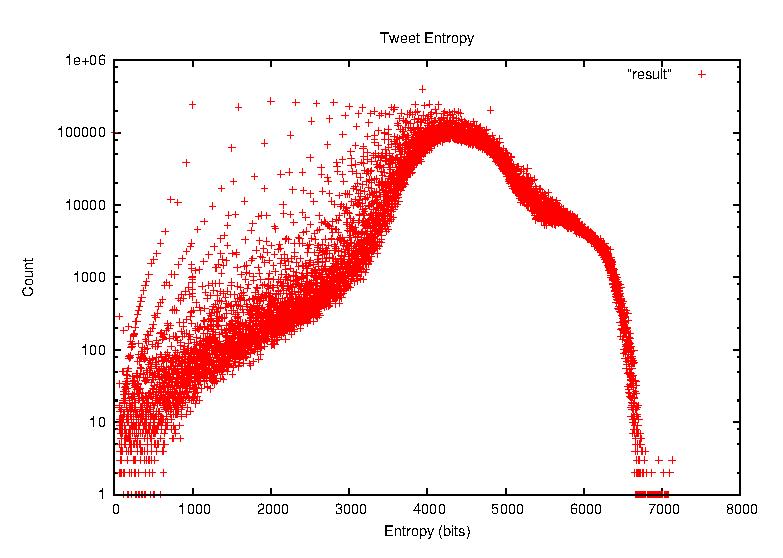
\includegraphics{text-entropy/result.eps}
\caption{Entropy distribution over tweets}
\label{entropy}
\end{figure}

We suspected entropy might vary per language, and so plotted entropy variation against the language field in \ref{entropyperlang}.

%\begin{figure}
%\centering
%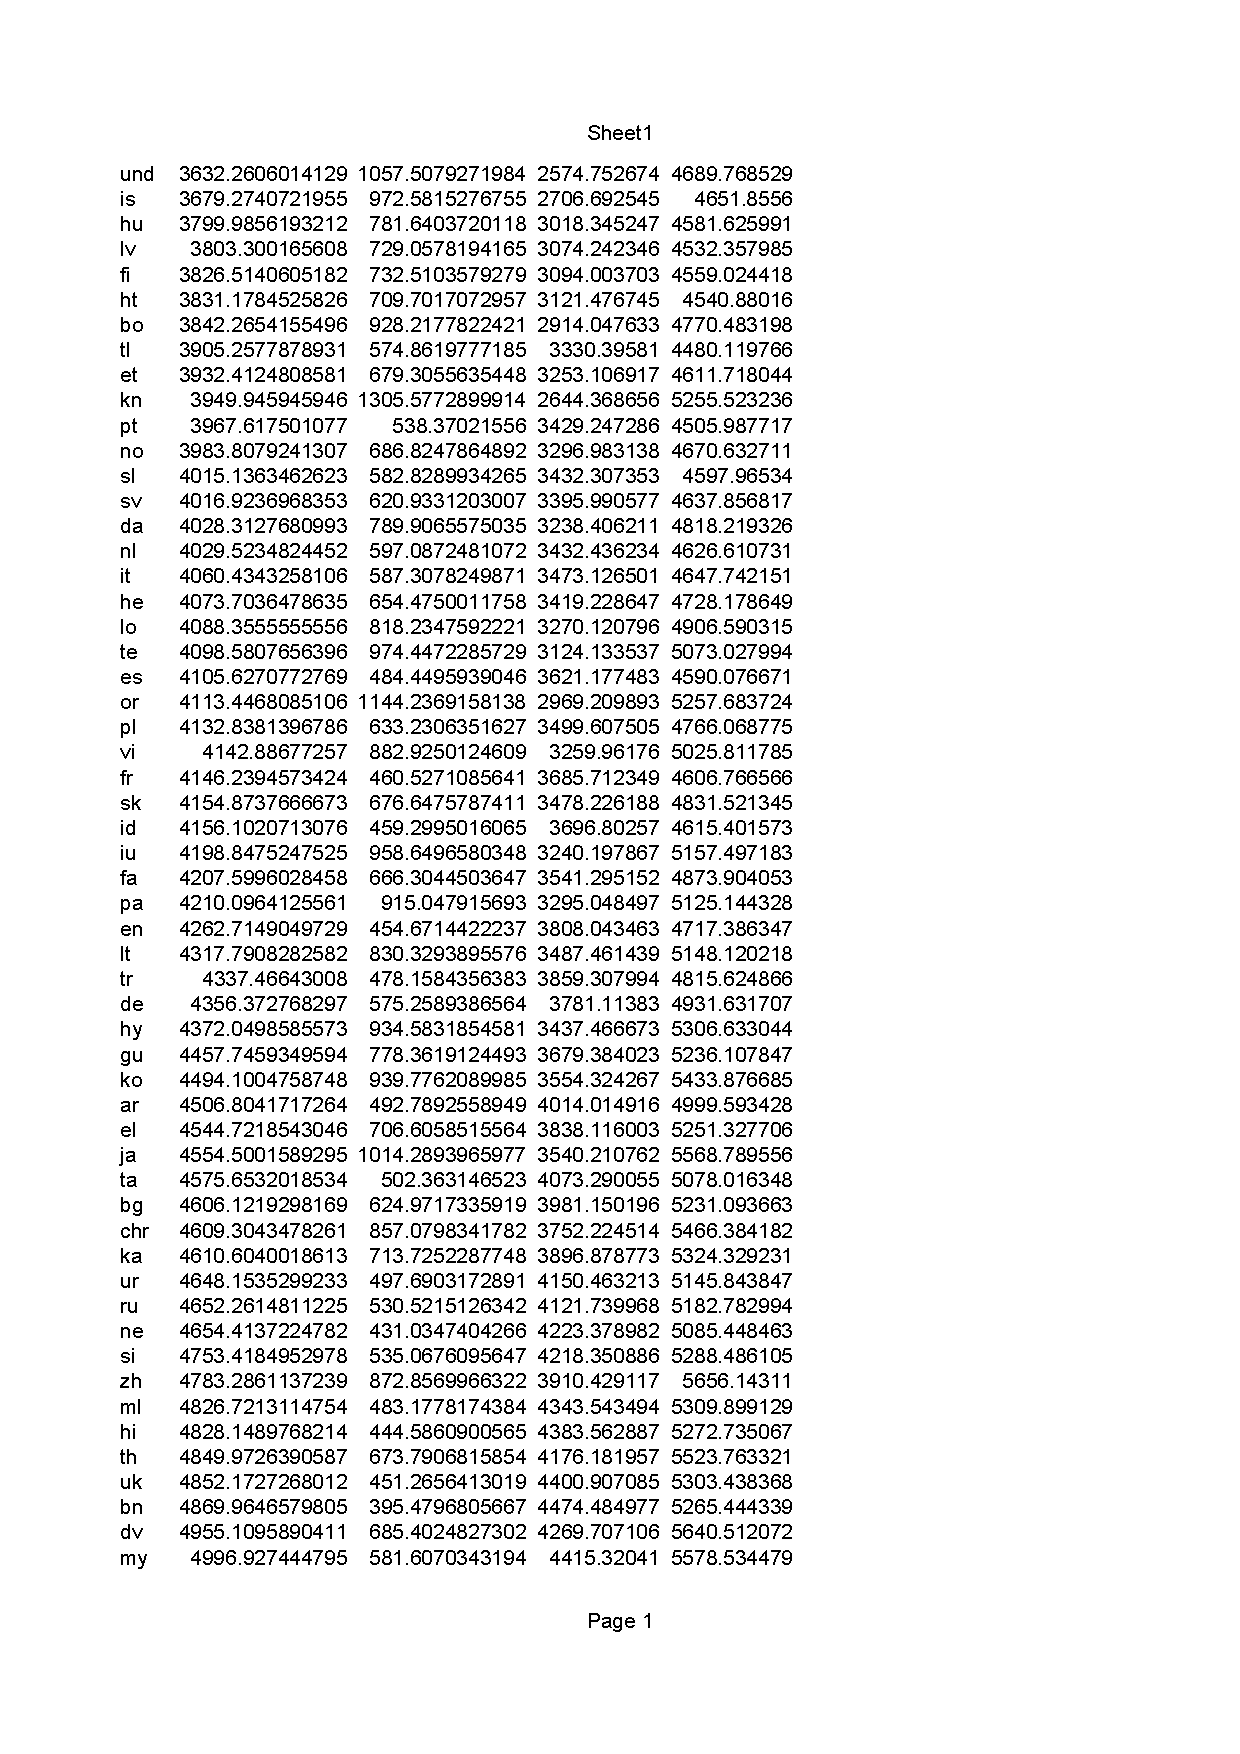
\includegraphics{text-entropy/entropyPerLang.pdf}
%\caption{Entropy distribution per language}
%\label{entropyperlang}
%\end{figure}

There are a few ouliers above 6.6 where we suspected we might find interesting content. The language count for these tweets is reported in \ref{highentropyperlang}. It is not surprising that among these outliers are ideogram-based languages, Japanese and Chinese.

\begin{table}
\centering
\begin{tabular}{|l|r||l|r|}
\hline
Lang & Count & Lang & Count \\
\hline
ja  & 2437 &  bg  &    2 \\
zh  & 58 & th   &   1 \\
en   &   12  & pa  &    1 \\
de   &   9 &   he  &    1 \\
ko    &  6 &  ar   &   1 \\
vi   &   3 & & \\
\hline
\end{tabular}
\caption{High Entropy Tweets per Language}
\end{table}

Recognizing base64 turned out to be harder than expected. Regex matching yielded a significant number of false positives.

We did, however, identify one odd pattern: sequences of nucleotids (ATGC letters) in long strings. We found a couple of users tweeting these sequences as ``Human DNA pieces''. While we initially thought this may be a covert communication channel, the sequences we tested turned out to be genuine human DNA, present in the publicly-available BLAST nucleotid database.


It is straightforward to encode bytes into groups of four nucleotids. With the 140-character twitter limit we can accomodate 35 bytes, or 280 bits, enough for our target bound.

For instance, assigning A,C,G,T the values 0,1,2,3, and writing every ascii value in base 4, lsb first, we can encode www.facebook.com as
\begin{verbatim}
CTCTCTCTCTCTGTGACGCGCGACCGATCGCC
CGAGCGTTCGTTCGGTGTGACGATCGTTCGTC
\end{verbatim}

Unfortunately this is not a very good disguise, as such a code
would exhibit strong self-correlation of order 2, where for actual genetic data an order 3 would be expected. This could be improved
by compressing or encrypting the data with a very simple scheme prior to encoding.


We attempted to match base64-encoded data with the heuristic of attempting a base64 decode, then keeping only the messages for which there is at least one ascii letter. Unfortunately this also produced too many false positives.



\subsection{Model building}

MapReduce is especially well fitted to compute the probability distributions over a Markov model. We will compute our models both on letters (n-grams) and tokenized words (for the english corpus only). We also need to test several tokenization models.As a part of n-gram model and tokenized words, a MapReduce program has been developed, the logic of the model follows
\begin{flushleft}

\begin{description}

\item[Mapper (n-gram)]

\begin{description}
\item[Input]: The twitter stream, without any pre-processing

\item[Functionality]: \begin{enumerate} 
          \item The twitter stream is parsed and the language field - 'Lang'	and Tweet text 'Text' gets extracted.
	\item The language fields is used according to the model that we are build [full one or English only]
          \item The tweet text further parsed into n-grams, without elimination of any bytes.
\end{enumerate}

\item[Output]: Each n-gram will be passed as a key to the reducer. The value is one. {n-gram, one}
\end{description}

\item[Mapper (tokenized words)]:

\begin{description}
\item[Input]: The twitter stream, without any pre-processing

\item[Functionality]: \begin{enumerate}
	\item  The twitter stream is parsed and the language field - 'Lang' and tweet text 'Text' gets extracted.
	\item The language fields is used according to the model that we are build [full one or English only]
	\item The tweet text further parsed into words, tweet texts always contains special characters,plural forms which should be eliminated. So regex pattern is used to extract only alpha-numeric characters
\end{enumerate} 

\item[Output]: Each word will be passed as a key to the reducer. The value is one. 
		{word, one}
			
\end{description}
	
\item[Reducer (common to n-grams and tokens)]:

\begin{description}
\item[Input]: {Key, Value}

\item[Functionality]: Count the Key

\item[Output]: Key Count
\end{description}

\end{description}
 
\end{flushleft}

We hit several trivial (in hindsight) difficulties that required model tweaking, and thus a lot of redundant computations. For the trigrams, the most common word was ``RT'': it is used as a marker at the beginning of a tweet to tag retweets. Thus, the model would mostly build strings of the ``RT'' word repeated. The second most common word was ``http'' followed closely by ``https''. For tokens, we (arbitrarily) excluded hashtags and user handles.

\paragraph{Entropy estimation}

Once the encoding channel is working, we shall make it run with random input bits, and measure on average how many bits fit in each tweet, for all our models (n-grams, english n-grams, english words). Combined with compression, we will estimate how many messages would be required for typical C\&C operations, checking in how many bits we can fit (for instance) a DDoS attack target or a typical shady url.

\paragraph{Detection}

The difficult part will be extracting suspicious messages conforming too well to our model. 

One first technique will be to use different Markov models of different orders, and see if for given accounts, their distribution of tweets follows a low-order model anormally better than a high-order one.

We will also use the n-gram table to compute likelihood for a set of hashtags, and try to extract randomly-generated hashtags from it. We will apply the same n-gram analysis to messages contents, and compare with the first naive regex-based classifier.

\section{Milestones}

\begin{description}
	\item[01.04.2014] Have a sample set of data ready in case the global collection effort does not work (MA), write a MapReduce implementation to build n-gram datasets (GR). Write MapReduce simple matchers (MA).
	\item[08.04.2014] Results from early assessment and detection
	\item[22.04.2014] Proof of concept for stealthy channel, MapReduce chain trimmer (GR), compressor/decompressor sample code (MA)
	\item[06.05.2014] Integrate final data sources and start looking for actual bots
	\item[13.05.2014] Final report 
\end{description}

\appendix

\paragraph{Channel building}

We propose to use an inverted form of Huffman coding to encode arbitrary bits into human-looking chains. The algorith wil work as follows:

First, prune the model to keep it down to a reasonable size, by excluding uncommon words.

Then, for every state in the chain, build a Huffman tree over the distribution for the next symbol.

To encode, begin with an empty starting state in the Markov chain. Perform a Huffman decoding operation on the tree of the current state, which will consume an arbitrary number of bits and produce a symbol. Output the symbol, compute the new state, and repeat until no bits are left, or the chain picks a terminating symbol, or the maximum output size is exceeded.

To decode, begin with the same empty state; for each token encoutered, perform Huffmann compression, repeat until the message is complete.

\section{Future Work}

Another option we want to consider (but less likely to give results) is encoding messages in deliberate grammar or orthography mistakes, trough permutation of simple characters. Decoding would be performed by a standard spell checker like aspell.



\section{Appendix A: results}

\begin{table}
\centering
\begin{tabular}{|l|r||l|r|}
\hline
Lang & Count & Lang & Count \\
\hline
en & 46324982 &             lt & 82100 \\
ja & 22399870 &             zh & 77609 \\
es & 15817824 &             no & 71175 \\
id & 10970703 &             fa & 69998 \\
ar & 9368831 &                      uk & 57837 \\
pt & 7189249 &                      he & 54388 \\
und & 3964165 &             ur & 37947 \\
tr & 3897656 &                      is & 35487 \\
fr & 2947715 &                      hi & 19889 \\
ru & 2566648 &                      ta & 8417 \\
tl & 1917014 &                      bn & 6140 \\
ko & 1730077 &                      ne & 5859 \\
th & 1664855 &                      hy & 2828 \\
it & 1029948 &                      ka & 2149 \\
nl & 1019123 &                      ml & 1159 \\
de & 725735 &                       te & 1071 \\
vi & 572220 &                       pa & 892 \\
et & 498251 &                       bo & 746 \\
pl & 453255 &                       si & 638 \\
sl & 429062 &                       my & 634 \\
ht & 350093 &                       iu & 505 \\
sk & 263615 &                       gu & 492 \\
sv & 248050 &                       kn & 444 \\
lv & 209531 &                       km & 433 \\
hu & 119744 &                       lo & 315 \\
bg & 115099 &                       am & 196 \\
el & 111589 &                       chr & 184 \\
fi & 110380 &                       dv & 146 \\
da & 110267 &                       or & 47 \\
\hline
\end{tabular}
\label{twperlang}
\caption{Tweets per language}
\end{table}

\end{document}
